\renewcommand{\leftmark}{INTRODUCTION}
\chapter{Introduction}\label{chap:intro}

L'objectif de ce mémoire est de concevoir une architecture réseau permettant la communications avec des capteurs/actuateurs utilisés pour la surveillances de cultures.

Ce déploiment a les caractéristiques suivantes:
\begin{itemize}
    \item Les noeuds du réseau sont fortement contraints énergétiquement. Ils seront typiquement alimentés
    par une batterie éventuellement associée à des panneaux solaires et un régulateur de charge.
    \item Les caractéristiques des liens radio LoRa et IEEE 802.15.4 sont différentes et susceptibles
    de changer au cours du temps suite à par exemple, la croissance des feuilles des cultures surveillées.
    \item Le débit des transmissions n'a pas besoin d'être élevé.
\end{itemize}

Actuellement, il existe une multitude de protocoles radio ayant chacun leurs caractéristiques.
La figure \ref{fig:intro-linkStandard} illustre le débit et la portée de différents protocoles.
%todo choix du protocoles: pas haut datarate et lora longue portée et 802.15.4 courte portée.

\begin{figure}
    \centering
    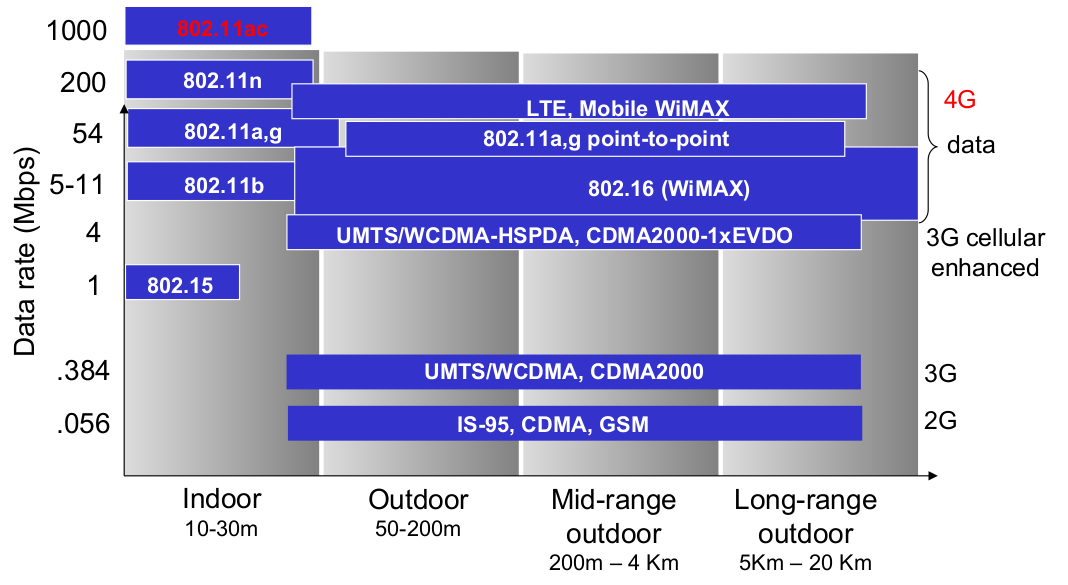
\includegraphics[scale=0.3]{res/link-standard.png}
    \label{fig:intro-linkStandard}
    \caption{Débits de données et distances de transmission.}
\end{figure}

Le choix d'une architecture hybride réalisée avec LoRa et 802.15.4 semble donc le plus approprié
pour ce déploiment.

La solution proposée est développée sur la plateforme RE-Mote de Zolertia.
Cette plateforme possède les caractéristiques suivantes:
% ARM Cortex-M3 32-Mhz
% 32KB de RAM
% I2C, SPI, UART
% General Purpose Pin(GPIO)
% USB 2.0 12 Mbps
%Micro-SD
%Built-in LiPo battery Charger
%RF 2.4Ghz ISM 2.4GHz IEEE802.15.4, 250 Kbps avec modulation DSSS
%ISM 863-868,915-, 920-, 950MHz